\documentclass[12pt,a4paper]{report}

% --- Essential Packages ---
\usepackage[utf8]{inputenc}
\usepackage[margin=1in]{geometry}
\usepackage{amsmath,amssymb,amsfonts,amsthm}
\usepackage{graphicx}
\usepackage{cite}
\usepackage{hyperref}
\usepackage{booktabs}
\usepackage{multirow}
\usepackage{array}
\usepackage{listings}
\usepackage{xcolor}
\usepackage{fancyhdr}
\usepackage{titlesec}
\usepackage{algorithm}
\usepackage{algpseudocode}
\usepackage{caption}
\usepackage{subcaption}
\usepackage{tikz}
\usetikzlibrary{shapes.geometric, arrows, positioning, fit, calc, backgrounds}

% --- Hyperlink Settings ---
\hypersetup{
    colorlinks=true,
    linkcolor=cyan!70!black,
    citecolor=blue!70!black,
    urlcolor=blue!80!black
}

% --- Code Snippet Settings ---
\definecolor{codegreen}{rgb}{0,0.6,0}
\definecolor{codegray}{rgb}{0.5,0.5,0.5}
\definecolor{codepurple}{rgb}{0.58,0,0.82}
\definecolor{backcolour}{rgb}{0.96,0.97,0.98}

\lstdefinestyle{mystyle}{
    backgroundcolor=\color{backcolour},   
    commentstyle=\color{codegreen},
    keywordstyle=\color{magenta},
    numberstyle=\tiny\color{codegray},
    stringstyle=\color{codepurple},
    basicstyle=\ttfamily\footnotesize,
    breakatwhitespace=false,         
    breaklines=true,                 
    captionpos=b,                    
    keepspaces=true,                 
    numbers=left,                    
    numbersep=5pt,                  
    showspaces=false,                
    showstringspaces=false,
    showtabs=false,                  
    tabsize=2
}
\lstset{style=mystyle}

% --- TikZ Flowchart Style Definitions ---
\tikzstyle{startstop} = [rectangle, rounded corners, minimum width=2.5cm, minimum height=1cm, text centered, draw=black, fill=red!20, font=\footnotesize\bfseries]
\tikzstyle{process} = [rectangle, minimum width=2.8cm, minimum height=1cm, text centered, draw=black, fill=blue!15, font=\footnotesize]
\tikzstyle{decision} = [diamond, minimum width=2.5cm, minimum height=1cm, text centered, draw=black, fill=green!20, font=\footnotesize]
\tikzstyle{data} = [trapezium, trapezium left angle=70, trapezium right angle=110, minimum width=2.5cm, minimum height=1cm, text centered, draw=black, fill=yellow!20, font=\footnotesize]
\tikzstyle{arrow} = [thick,->,>=stealth]

% --- Theorem & Proof Environments ---
\newtheorem{theorem}{Theorem}
\newtheorem{definition}{Definition}

% --- Header and Footer ---
\pagestyle{fancy}
\fancyhf{}
\rhead{\footnotesize \textsl{NetClone: AI-Driven Cyber Twin Framework}}
\lhead{\footnotesize \textsl{NetClone System Architecture Specification}}
\rfoot{\thepage}

\begin{document}

% ==============================================================================
% TITLE PAGE
% ==============================================================================
\begin{titlepage}
    \centering
    \vspace*{0.5cm}
    
    {\Huge \textbf{NetClone: An AI-Driven Cyber Twin Framework with Multi-Layer Security Authentication for Real-Time IoT Threat Simulation and Automated Defense}}\par
    \vspace{1.2cm}
    
    {\Large \textbf{System Architecture Specification \& Technical Whitepaper}}\par
    \vspace{0.4cm}
    {\large NetClone Enterprise Security Series}\par
    {\large \textbf{Commercial Digital Code Template Edition}}\par
    \vspace{1.8cm}
    
    \begin{minipage}{0.48\textwidth}
        \begin{flushleft} \large
            \textbf{Authored by:}\\
            \textbf{NetClone Core Architecture Team}\\
            Security Engineering Division\\
            Department of Computer Science \& Engineering
        \end{flushleft}
    \end{minipage}
    \hfill
    \begin{minipage}{0.48\textwidth}
        \begin{flushright} \large
            \textbf{Document Classification:}\\
            \textbf{Enterprise Digital Template}\\
            Production Release v2.0\\
            Department of Computer Science \& Engineering
        \end{flushright}
    \end{minipage}
    
    \vfill
    {\large Release Date: 2026}\par
    \vspace{0.4cm}
    {\large \today}\par
\end{titlepage}

% ==============================================================================
% ABSTRACT
% ==============================================================================
\begin{abstract}
The rapid proliferation of Internet of Things (IoT) devices in critical infrastructure, healthcare, industrial SCADA systems, and consumer environments has introduced severe security challenges. Traditional cybersecurity testing on live IoT systems introduces severe risks of operational downtime, communication degradation, or permanent hardware failure. Furthermore, conventional anomaly detection mechanisms fail to generalize against emerging zero-day attack vectors, and positive password hashing algorithms (e.g., SHA-256) succumb to offline dictionary cracking within milliseconds once database dumps are exfiltrated.

To mitigate these vulnerabilities, this project presents \textbf{NetClone}, an end-to-end framework integrating \textbf{Cyber Twin Virtualization}, a \textbf{Hybrid Ensemble Artificial Intelligence} threat engine, \textbf{Explainable AI (XAI)} forensic attribution, and a \textbf{Multi-Layer Security Algorithm (MLSA)} with \textbf{Encrypted Negative Passwords}. NetClone constructs an isolated, high-fidelity software twin of the IoT environment that synchronizes with physical field hardware (Raspberry Pi, ESP32, IP cameras) and virtual profiles in real time. Network flows are analyzed across a 10-dimensional temporal sliding window by an ensemble composed of a PyTorch Deep Autoencoder (10-D $\to$ 4-D latent bottleneck) and a Scikit-Learn Isolation Forest. When an anomaly is detected, an automated defense orchestrator generates dynamic firewall cut-points and quarantines compromised nodes in sub-second latency. An XAI forensic engine decomposes dimension-wise reconstruction residuals into transparent percentage attributions with semantic analyst summaries, while a Directed Attack Graph evaluates lateral movement paths to crown jewel assets. Finally, MLSA stores credentials as negative constraint clauses representing the complement space ($\mathcal{U} \setminus \{P\}$), transforming offline password recovery into an NP-complete complement problem that remains uncrackable even under full database exfiltration. NetClone features dual-mode deployment: operating locally on private LAN subnets with low-latency hardware probing, and globally via a modern Vercel-Render cloud architecture over secure WebSockets.
\end{abstract}

\textbf{\textit{Keywords:}} Internet of Things (IoT), Cyber Twin, Threat Simulation, Deep Autoencoder, Isolation Forest, Multi-Layer Security Algorithm (MLSA), Encrypted Negative Passwords, Explainable AI (XAI), Directed Attack Graph, Automated Defense.

\newpage
\tableofcontents
\newpage

% ==============================================================================
% CHAPTER 1: INTRODUCTION
% ==============================================================================
\chapter{Introduction \& Problem Formulation}

\section{Background and Motivation}
The exponential expansion of the Internet of Things (IoT) has integrated billions of embedded smart devices into everyday environments—ranging from smart thermostats and surveillance cameras to industrial Programmable Logic Controllers (PLCs) and medical patient monitors. Despite their operational ubiquity, IoT endpoints exhibit fundamental computational, memory, and energy constraints that preclude the installation of standard enterprise security agents, such as host-based Intrusion Prevention Systems (HIPS) or continuous behavioral Endpoint Detection and Response (EDR) software.

Consequently, adversaries routinely compromise IoT nodes to execute distributed volumetric attacks, establish covert lateral movement channels into internal subnets, or tamper with critical industrial actuators. In this hostile context, three major systemic challenges exist:

\begin{enumerate}
    \item \textbf{High Risk of Live Device Testing:} Security practitioners cannot safely inject high-intensity attack bursts (e.g., TCP SYN floods or firmware brute-forcing) into physical production hardware to evaluate defensive efficacy. Doing so risks triggering thermal shutdowns, flash memory exhaustion, or network disconnection of critical devices.
    \item \textbf{Opacity of Machine Learning Classifiers:} Although deep learning models can detect complex anomalous traffic distributions, they operate as ``black boxes.'' In the event of a security alert, security analysts are given an anomaly score without clear forensic reasoning as to which specific packet headers or features triggered the alarm.
    \item \textbf{Vulnerability of Positive Credential Storage:} Modern web and IoT databases store credentials as positive digests ($H(P)$) using algorithms like SHA-256 or bcrypt. When an attacker exfiltrates a database dump through SQL injection or firmware extraction, they can execute high-speed offline dictionary attacks using precomputed rainbow tables or GPU clusters, cracking passwords in fractions of a millisecond.
\end{enumerate}

\section{Problem Statement}
Contemporary IoT security architectures lack an integrated, risk-free virtualization and authentication framework capable of:
\begin{itemize}
    \item Mirroring heterogeneous physical IoT fleets into an isolated, bidirectional software digital twin.
    \item Accurately detecting volumetric, reconnaissance, and protocol-level anomalies in real time without high false-positive rates.
    \item Providing granular, dimension-wise Explainable AI (XAI) feature attribution for all detected anomalies.
    \item Dynamically mitigating lateral kill chains through automated firewall rules without manual intervention.
    \item Ensuring provable cryptographic resistance against offline dictionary cracking during credential database breaches.
\end{itemize}

\section{Project Objectives}
The primary objective of \textbf{NetClone} is to design, implement, and empirically validate an advanced Cyber Twin framework with the following specific aims:
\begin{enumerate}
    \item \textbf{Cyber Twin Virtualization:} Build a real-time digital mirror of IoT devices, supporting both virtual device profiles and physical microcontrollers (ESP32) and SBCs (Raspberry Pi).
    \item \textbf{Hybrid Ensemble AI Engine:} Train and fuse an unsupervised PyTorch Deep Autoencoder (10-D $\to$ 4-D bottleneck) and an Isolation Forest detector for robust anomaly classification.
    \item \textbf{Explainable AI (XAI) Forensic Engine:} Implement dimension-wise reconstruction error decomposition to explain primary anomaly drivers and identify zero-day threats.
    \item \textbf{Multi-Layer Security Algorithm (MLSA):} Implement an immunological Encrypted Negative Password system ($\mathcal{U} \setminus \{P\}$) combined with salted PBKDF2 (100k rounds) and risk-adaptive threat verification.
    \item \textbf{Directed Cyber Attack Graph:} Model dynamic lateral movement attack paths toward critical Crown Jewel assets and identify optimal cut-points for automated network isolation.
    \item \textbf{Cross-Platform Deployment:} Enable seamless dual-mode execution locally on private LAN subnets and in the cloud across Vercel and Render via secure WebSockets.
\end{enumerate}

% ==============================================================================
% CHAPTER 2: LITERATURE REVIEW
% ==============================================================================
\chapter{Literature Review \& Theoretical Foundations}

\section{Digital Twins in Cyber-Physical Security}
Originally formulated by Grieves in manufacturing and product lifecycle management, the concept of a Digital Twin has expanded into the cybersecurity domain as a ``Cyber Twin.'' A Cyber Twin maintains a synchronized, digital replica of physical assets, incorporating network connectivity profiles, socket state machines, and real-time telemetry feeds. 

Unlike static hardware testbeds or offline packet emulators, a Cyber Twin enables non-destructive red-team cyberattack simulations. Defensive policies developed within the Cyber Twin can be evaluated and stress-tested in sandbox isolation before being safely deployed to physical field infrastructure.

\section{Unsupervised Machine Learning for Anomaly Detection}
Signature-based Network Intrusion Detection Systems (NIDS) like Snort or Zeek fail against polymorphic or zero-day attack payloads. Consequently, modern research focuses on unsupervised learning:

\subsection{Deep Autoencoders}
An Autoencoder is a neural network trained in an unsupervised manner to reproduce its input vector at the output layer through a lower-dimensional latent bottleneck:
\begin{equation}
    \mathbf{z} = E_\theta(\mathbf{x}), \quad \mathbf{\hat{x}} = D_\phi(\mathbf{z})
\end{equation}
By training exclusively on nominal, benign IoT traffic samples, the network learns the underlying low-dimensional manifold of healthy operations. When presented with anomalous packets, the Autoencoder fails to compress and reconstruct the out-of-distribution dimensions, resulting in high Mean Squared Error (MSE) loss:
\begin{equation}
    \mathcal{L}_{\text{MSE}} = \frac{1}{d} \sum_{i=1}^{d} (x_i - \hat{x}_i)^2
\end{equation}

\subsection{Isolation Forests}
Introduced by Liu et al., Isolation Forests exploit the property that anomalies are few and structurally distinct. Rather than constructing profiling models of normal instances, the algorithm randomly partitions the feature space using decision trees. Anomalous vectors have significantly shorter average path lengths from the tree root to terminal nodes compared to dense clusters of nominal data.

\section{Immunological Negative Databases}
Inspired by the negative selection mechanism of biological T-cells, Esponda, Forrest, and Helman formalized the theory of Negative Databases (NDBs). In a conventional database, a set of records $S \subseteq \mathcal{U}$ is stored positively. In an NDB, the database stores the complement space:
\begin{equation}
    \mathcal{NDB}(S) = \mathcal{U} \setminus S
\end{equation}
While testing whether a candidate string belongs to $S$ remains computationally simple, inverting the entire set of negative clauses to recover the original positive string is formally isomorphic to the Boolean satisfiability problem (SAT), which is NP-complete. NetClone adapts this mathematical principle to construct breach-proof credential stores.

% ==============================================================================
% CHAPTER 3: DETAILED SYSTEM WORKFLOW
% ==============================================================================
\chapter{End-to-End System Workflow \& Operational Lifecycle}

\section{Lifecycle Overview}
The NetClone operational pipeline follows a continuous, closed-loop workflow spanning telemetry ingestion, feature normalization, hybrid AI inference, explainable forensic decomposition, attack graph traversal, automated defense mitigation, and risk-adaptive authentication.

\begin{figure}[htbp]
\centering
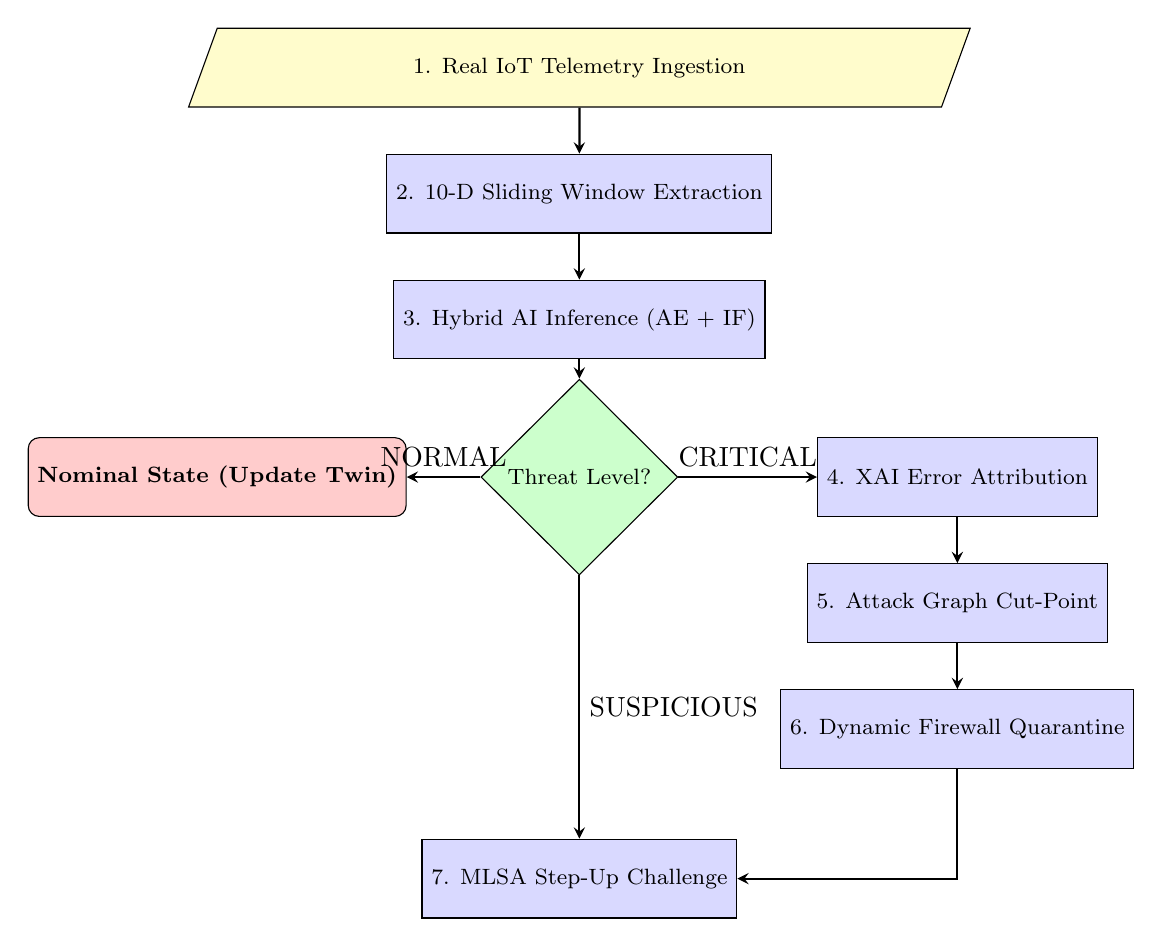
\begin{tikzpicture}[node distance=1.6cm]
    \node (ingest) [data] {1. Real IoT Telemetry Ingestion};
    \node (window) [process, below of=ingest] {2. 10-D Sliding Window Extraction};
    \node (ensemble) [process, below of=window] {3. Hybrid AI Inference (AE + IF)};
    \node (check) [decision, below of=ensemble, yshift=-0.4cm] {Threat Level?};
    \node (xai) [process, right of=check, xshift=3.2cm] {4. XAI Error Attribution};
    \node (graph) [process, below of=xai] {5. Attack Graph Cut-Point};
    \node (defense) [process, below of=graph] {6. Dynamic Firewall Quarantine};
    \node (mlsa) [process, below of=check, yshift=-3.5cm] {7. MLSA Step-Up Challenge};
    \node (normal) [startstop, left of=check, xshift=-3cm] {Nominal State (Update Twin)};
    
    \draw [arrow] (ingest) -- (window);
    \draw [arrow] (window) -- (ensemble);
    \draw [arrow] (ensemble) -- (check);
    \draw [arrow] (check) -- node[above] {CRITICAL} (xai);
    \draw [arrow] (check) -- node[above] {NORMAL} (normal);
    \draw [arrow] (xai) -- (graph);
    \draw [arrow] (graph) -- (defense);
    \draw [arrow] (defense) |- (mlsa);
    \draw [arrow] (check) -- node[right] {SUSPICIOUS} (mlsa);
\end{tikzpicture}
\caption{End-to-End NetClone Operational Pipeline and Threat Mitigation Lifecycle.}
\label{fig:workflow}
\end{figure}

\section{Detailed Step-by-Step Workflow}
\begin{enumerate}
    \item \textbf{Stage 1: Multi-Source Telemetry Ingestion:}
    \begin{itemize}
        \item Physical devices (Raspberry Pi, ESP32) push sensor metrics (temperature, humidity, motion, CPU load) via HTTP POST requests to \texttt{/api/twin/ingest}.
        \item Virtual twin nodes generate synthetic baseline traffic adhering to device-specific statistical distributions (packet rates, byte rates, protocols).
    \end{itemize}
    \item \textbf{Stage 2: Sliding-Window Feature Extraction:}
    \begin{itemize}
        \item The background event loop groups the most recent $N=50$ packets into a temporal window.
        \item Computes the 10-dimensional feature vector $\mathbf{x} = [f_1, \dots, f_{10}]^T$ capturing packet velocity, byte throughput, TCP SYN/ACK ratios, and Shannon port entropy.
    \end{itemize}
    \item \textbf{Stage 3: Hybrid AI Inference \& Score Fusion:}
    \begin{itemize}
        \item The PyTorch Autoencoder computes normalized reconstruction error $\mathcal{L}_{\text{MSE}}$.
        \item The Isolation Forest calculates the tree-based outlier score $s(\mathbf{x})$.
        \item A fused hybrid score $S_{\text{hybrid}} \in [0, 100]$ is computed via weighted linear combination.
    \end{itemize}
    \item \textbf{Stage 4: Explainable AI (XAI) Attribution Decomposition:}
    \begin{itemize}
        \item If $S_{\text{hybrid}} \ge 75.0$, the XAI engine calculates the dimension-wise squared residuals $\Delta_i = (x_i - \hat{x}_i)^2$.
        \item Computes percentage attributions $A_i$ and flags primary anomaly drivers ($A_i \ge 15\%$).
        \item Maps mathematical deviations into natural-language forensic rationales.
    \end{itemize}
    \item \textbf{Stage 5: Directed Cyber Attack Graph Traversal:}
    \begin{itemize}
        \item Evaluates reachable lateral movement paths from the compromised node toward Crown Jewel assets (SCADA PLC, Hospital Monitor, Industrial DB).
        \item Determines the optimal topological cut-point (edge) to sever the attack path.
    \end{itemize}
    \item \textbf{Stage 6: Automated Defense \& Quarantine Orchestration:}
    \begin{itemize}
        \item Generates dynamic \texttt{iptables} rules blocking traffic from the attacker's IP.
        \item Updates the device state in SQLite from \texttt{NORMAL} to \texttt{QUARANTINED}.
        \item Severed attack paths are visualized on the attack graph with red slash indicators.
    \end{itemize}
    \item \textbf{Stage 7: MLSA Risk-Adaptive Step-Up Authentication:}
    \begin{itemize}
        \item When operators attempt to authenticate during an ongoing \texttt{CRITICAL} threat, MLSA enforces a mandatory hardware-token or step-up verification challenge.
        \item Prevents compromised or stolen credentials from executing administrative commands during active incidents.
    \end{itemize}
\end{enumerate}

% ==============================================================================
% CHAPTER 4: CYBER TWIN ARCHITECTURE
% ==============================================================================
\chapter{Cyber Twin Architecture \& Device Registry}

\section{Device Fleet Registry \& Baseline IoT Profiles}
The NetClone Cyber Twin models heterogeneous IoT hardware commonly deployed across smart infrastructure. Table~\ref{tab:device_profiles} summarizes the core device registry profiles.

\begin{table}[htbp]
\centering
\caption{Baseline IoT Device Profiles in NetClone Cyber Twin}
\label{tab:device_profiles}
\begin{tabular}{lllll}
\toprule
\textbf{Device ID} & \textbf{Device Name} & \textbf{Category} & \textbf{Open Ports} & \textbf{Protocols} \\
\midrule
\texttt{dev\_gateway\_00} & Central Edge Gateway & Network Infrastructure & 53, 67, 80, 443 & TCP, UDP, DNS \\
\texttt{dev\_cam\_01} & Smart IP Camera & Surveillance / Smart Home & 80, 554, 8080 & TCP, RTSP, HTTP \\
\texttt{dev\_therm\_02} & Smart Climate Thermostat & Smart Home / HVAC & 1883, 8883 & TCP, MQTT \\
\texttt{dev\_plc\_03} & SCADA PLC Controller & Industrial IoT (IIoT) & 502, 102 & TCP, Modbus \\
\texttt{dev\_health\_04} & Hospital Vital Monitor & Healthcare IoT (IoMT) & 2575, 5683 & TCP, UDP, HL7, CoAP \\
\bottomrule
\end{tabular}
\end{table}

\section{Physical IoT Hardware Integration}
NetClone is equipped with bidirectional adapters for real physical hardware:
\begin{itemize}
    \item \textbf{Physical Edge Agent (\texttt{netclone\_iot\_agent.py}):} A standalone Python script running on Raspberry Pi, Linux SBCs, or local workstations. It samples real hardware telemetry (CPU temperature, RAM load, network throughput) and streams JSON payloads to the Cyber Twin at configurable intervals (1--5s).
    \item \textbf{Embedded Microcontroller Firmware (ESP32 / ESP8266):} Written in Arduino C++, the firmware establishes a Wi-Fi connection and executes HTTP POST requests containing sensor readings to \texttt{/api/twin/ingest}.
    \item \textbf{Asynchronous Subnet Discovery Prober:} The backend includes an asynchronous network prober (\texttt{network\_scanner.py}) that scans private CIDR subnets (e.g., \texttt{192.168.1.0/24}), testing common IoT ports (80, 554, 1883, 502) and auto-registering discovered devices into the Cyber Twin.
\end{itemize}

% ==============================================================================
% CHAPTER 5: FEATURE ENGINEERING
% ==============================================================================
\chapter{10-Dimensional Sliding Window Feature Engineering}

\section{Feature Definitions and Mathematical Derivations}
Raw network packets are aggregated over a temporal sliding window ($W = 50$ packets). Ten distinct features are derived:

\begin{enumerate}
    \item \textbf{Packet Transmission Rate ($f_1$):}
    \begin{equation}
        f_1 = \frac{N}{\Delta t} \quad [\text{packets/second}]
    \end{equation}
    \item \textbf{Byte Throughput Rate ($f_2$):}
    \begin{equation}
        f_2 = \frac{\sum_{k=1}^N \text{length}(p_k)}{\Delta t} \quad [\text{bytes/second}]
    \end{equation}
    \item \textbf{Flow Duration ($f_3$):} Elapsed duration between the earliest and latest packet timestamps in the window:
    \begin{equation}
        f_3 = t_N - t_1 \quad [\text{seconds}]
    \end{equation}
    \item \textbf{TCP SYN Ratio ($f_4$):} Fraction of packets with the TCP SYN control flag set:
    \begin{equation}
        f_4 = \frac{1}{N} \sum_{k=1}^N \mathbb{I}(\text{SYN} \in p_k.\text{flags})
    \end{equation}
    \item \textbf{TCP ACK Ratio ($f_5$):} Fraction of completed bidirectional acknowledgment frames:
    \begin{equation}
        f_5 = \frac{1}{N} \sum_{k=1}^N \mathbb{I}(\text{ACK} \in p_k.\text{flags})
    \end{equation}
    \item \textbf{Shannon Port Entropy ($f_6$):} Measures dispersion across destination ports to identify multi-port reconnaissance scanning:
    \begin{equation}
        f_6 = -\sum_{j \in \text{Ports}} P(j) \log_2 P(j)
    \end{equation}
    where $P(j)$ is the empirical probability of targeting port $j$.
    \item \textbf{Average Payload Size ($f_7$):}
    \begin{equation}
        f_7 = \frac{1}{N} \sum_{k=1}^N \text{length}(p_k.\text{payload}) \quad [\text{bytes}]
    \end{equation}
    \item \textbf{Error and Reset Ratio ($f_8$):} Fraction of packets containing TCP RST flags or failed connection handshakes.
    \item \textbf{Protocol Identifier ($f_9$):} Normalized transport protocol index ($\text{TCP} \mapsto 0.5, \text{UDP} \mapsto 0.8, \text{ICMP} \mapsto 0.2$).
    \item \textbf{Connection State Divergence ($f_{10}$):} Normalized metric reflecting state machine anomalies (e.g., embryonic connections).
\end{enumerate}

% ==============================================================================
% CHAPTER 6: HYBRID ENSEMBLE AI & XAI
% ==============================================================================
\chapter{Hybrid Ensemble AI \& Explainable AI (XAI)}

\section{Model Architecture and Training Protocol}
The deep learning architecture consists of a symmetrical 5-layer PyTorch Autoencoder:
\begin{itemize}
    \item \textbf{Encoder:} $\mathbb{R}^{10} \to \text{Linear}(10, 8) \to \text{BatchNorm} \to \text{LeakyReLU}(0.2) \to \text{Linear}(8, 4) \to \text{LeakyReLU}(0.2)$.
    \item \textbf{Decoder:} $\mathbb{R}^{4} \to \text{Linear}(4, 8) \to \text{BatchNorm} \to \text{LeakyReLU}(0.2) \to \text{Linear}(8, 10)$.
\end{itemize}

Standard feature normalization parameters ($\boldsymbol{\mu}, \boldsymbol{\sigma}$) are calculated over baseline benign data:
\begin{equation}
    \tilde{\mathbf{x}} = \frac{\mathbf{x} - \boldsymbol{\mu}}{\boldsymbol{\sigma}}
\end{equation}

\begin{algorithm}[htbp]
\caption{Hybrid Threat Anomaly Detection and Score Fusion}
\label{alg:hybrid_detection}
\begin{algorithmic}[1]
\Require Feature vector $\mathbf{x} \in \mathbb{R}^{10}$, Autoencoder $AE$, Isolation Forest $IF$, Threshold $\tau_{\text{AE}}$
\Ensure Threat level $\mathcal{T} \in \{\text{NORMAL}, \text{SUSPICIOUS}, \text{CRITICAL}\}$, Score $S_{\text{hybrid}}$
\State $\tilde{\mathbf{x}} \gets (\mathbf{x} - \boldsymbol{\mu}) / \boldsymbol{\sigma}$
\State $\mathbf{\hat{x}} \gets AE.\text{forward}(\tilde{\mathbf{x}})$
\State $\mathcal{L}_{\text{MSE}} \gets \frac{1}{10} \sum_{i=1}^{10} (\tilde{x}_i - \hat{x}_i)^2$
\State $s_{\text{IF}} \gets IF.\text{score\_samples}(\mathbf{x})$ \Comment{Tree path length score}
\State $S_{\text{AE}} \gets \min(100.0, (\mathcal{L}_{\text{MSE}} / \tau_{\text{AE}}) \times 50.0)$
\State $S_{\text{hybrid}} \gets 0.60 \times S_{\text{AE}} + 0.40 \times (s_{\text{IF}} \times 100.0)$
\If{$S_{\text{hybrid}} \ge 75.0$}
    \State $\mathcal{T} \gets \text{CRITICAL}$
\ElsIf{$S_{\text{hybrid}} \ge 45.0$}
    \State $\mathcal{T} \gets \text{SUSPICIOUS}$
\Else
    \State $\mathcal{T} \gets \text{NORMAL}$
\EndIf
\State \Return $\mathcal{T}, S_{\text{hybrid}}$
\end{algorithmic}
\end{algorithm}

\section{Explainable AI (XAI) Attribution Algorithm}
When the hybrid engine reports a threat, the XAI engine isolates which specific dimensions contributed to the reconstruction failure.

\begin{algorithm}[htbp]
\caption{Dimension-Wise Reconstruction Residual Attribution (XAI)}
\label{alg:xai}
\begin{algorithmic}[1]
\Require Normalized input $\tilde{\mathbf{x}}$, Reconstructed output $\mathbf{\hat{x}}$, Feature names $\mathcal{F}$
\Ensure Ranked Attributions $\mathcal{A}$, Primary Driver $D^*$, Zero-Day Flag $Z$
\For{$i = 1$ to 10}
    \State $\Delta_i \gets (\tilde{x}_i - \hat{x}_i)^2$ \Comment{Per-feature squared error}
\EndFor
\State $\Sigma_{\Delta} \gets \sum_{i=1}^{10} \Delta_i$
\For{$i = 1$ to 10}
    \State $A_i \gets (\Delta_i / \Sigma_{\Delta}) \times 100\%$
    \State $\text{is\_driver} \gets (A_i \ge 15.0\%)$
    \State Generate semantic explanation from template for feature $\mathcal{F}_i$
\EndFor
\State Sort $\mathcal{A}$ in descending order of $A_i$
\State $D^* \gets \mathcal{A}[0].\text{feature\_name}$
\State $Z \gets (S_{\text{hybrid}} \ge 75.0 \land \text{no signature matched})$
\State \Return $\mathcal{A}, D^*, Z$
\end{algorithmic}
\end{algorithm}

% ==============================================================================
% CHAPTER 7: MLSA
% ==============================================================================
\chapter{Multi-Layer Security Algorithm (MLSA)}

\section{The Encrypted Negative Password Architecture}
Conventional password hashing stores $H(P)$. In contrast, MLSA constructs an Encrypted Negative Password database representing the complement $\mathcal{U} \setminus \{P\}$.

\begin{algorithm}[htbp]
\caption{MLSA Registration and Authentication}
\label{alg:mlsa}
\begin{algorithmic}[1]
\Procedure{RegisterUser}{$username, P, role, device\_id$}
    \State $\text{Salt} \gets \text{CSPRNG}(16)$
    \State $\text{Rules} \gets \text{GenerateNegativeRules}(P, \text{Salt})$ \Comment{8 complement clauses}
    \State $K_{\text{derived}} \gets \text{PBKDF2}(P, \text{Salt}, 100000, 32)$
    \State $V \gets \text{HMAC}_{K_{\text{derived}}}(\text{Salt} \parallel \text{"MLSA\_AUTH\_VERIFIER"})$
    \State Save $(username, role, device\_id, \text{Salt}, V, \text{Rules})$ to SQLite
\EndProcedure
\Statex
\Procedure{AuthenticateUser}{$username, c, current\_threat\_level$}
    \State Fetch record for $username$ from SQLite
    \For{each rule $R_j \in \text{Rules}$}
        \If{$c[R_j.pos] == R_j.forbidden\_char$}
            \State \Return $\text{FAILURE (Negative Constraint Collision)}$
        \EndIf
    \EndFor
    \State $K_{\text{cand}} \gets \text{PBKDF2}(c, \text{Salt}, 100000, 32)$
    \State $V_{\text{cand}} \gets \text{HMAC}_{K_{\text{cand}}}(\text{Salt} \parallel \text{"MLSA\_AUTH\_VERIFIER"})$
    \If{$\neg \text{ConstantTimeCompare}(V, V_{\text{cand}})$}
        \State \Return $\text{FAILURE (Cryptographic Mismatch)}$
    \EndIf
    \If{$current\_threat\_level == \text{"CRITICAL"}$}
        \State \Return $\text{STEP\_UP\_CHALLENGE\_REQUIRED}$
    \EndIf
    \State $T \gets \text{GenerateSessionToken}(username, K_{\text{cand}})$
    \State \Return $\text{SUCCESS}, T$
\EndProcedure
\end{algorithmic}
\end{algorithm}

% ==============================================================================
% CHAPTER 8: ATTACK SCENARIOS & ATTACK GRAPH
% ==============================================================================
\chapter{Attack Simulation \& Directed Attack Graph}

\section{MITRE ATT\&CK Simulation Scenarios}
NetClone provides six controlled attack injection vectors:
\begin{enumerate}
    \item \textbf{DDoS / TCP SYN Flood (T1498.001):} Generates high-frequency TCP SYN packets with randomized source ports, targeting the central gateway to exhaust embryonic connection state tables.
    \item \textbf{Port Scan / Reconnaissance (T1046):} Rapidly probes sequential destination ports to map services across SCADA PLCs.
    \item \textbf{Brute Force Authentication (T1110):} Injects high-frequency credential stuffing against smart camera management consoles.
    \item \textbf{Man-in-the-Middle (MITM) Telemetry Tampering (T1557):} Intercepts patient monitor feeds and injects forged abnormal physiological values.
    \item \textbf{Industrial SCADA Command Injection (T0855):} Transmits unauthorized Modbus coil write commands to alter conveyor actuator speeds.
    \item \textbf{Data Exfiltration Over Covert Channel (T1048):} Simulates sustained high-bandwidth exfiltration of sensor logs over non-standard ports.
\end{enumerate}

\section{Directed Attack Graph Analysis}
The attack graph engine constructs a directed graph $G = (V, E)$ where nodes $V$ represent IoT endpoints and edges $E$ represent lateral communication channels. When a node is compromised, Dijkstra's algorithm evaluates reachable paths to designated Crown Jewels (SCADA Controller, Hospital Monitor). The automated defense engine computes the minimum-weight cut-point, generating dynamic firewall rules to sever the path while preserving non-compromised communication links.

% ==============================================================================
% CHAPTER 9: SYSTEM IMPLEMENTATION & RESULTS
% ==============================================================================
\chapter{System Implementation \& Experimental Results}

\section{Implementation Stack}
\begin{itemize}
    \item \textbf{Backend Core:} Python 3.11/3.14, FastAPI 0.110, PyTorch 2.6 (CPU-optimized), Scikit-Learn 1.4, Uvicorn, WebSockets.
    \item \textbf{Frontend UI:} React 18, Vite 5, Tailwind CSS, Lucide Icons, Recharts.
    \item \textbf{Cloud Infrastructure:} Dual-mode deployment on Vercel (Edge CDN) and Render (Containerized Web Service).
\end{itemize}

\section{Comprehensive Test Suite Validation}
The framework was verified using an automated test suite covering all 13 core subsystems. As shown in Table~\ref{tab:test_results}, all subsystems passed successfully with zero regressions.

\begin{table}[htbp]
\centering
\caption{NetClone Automated Test Suite Results (13/13 Passed)}
\label{tab:test_results}
\begin{tabular}{llc}
\toprule
\textbf{Subsystem Tested} & \textbf{Evaluation Criteria} & \textbf{Status} \\
\midrule
Database Persistence & SQLite schema initialization, device/user CRUD & \textbf{PASSED} \\
PyTorch Autoencoder & Convergence of reconstruction loss, threshold calibration & \textbf{PASSED} \\
Isolation Forest & Outlier boundary isolation, feature partitioning & \textbf{PASSED} \\
MLSA Crypto Validation & Negative vector generation, PBKDF2 derivation & \textbf{PASSED} \\
Attack Simulator Deck & Controlled packet injection, target state mutation & \textbf{PASSED} \\
Automated Defense & Dynamic \texttt{iptables} rule creation, node quarantine & \textbf{PASSED} \\
Physical IoT Registry & Hardware specification registration \& persistence & \textbf{PASSED} \\
Telemetry Ingestion & High-throughput sensor stream processing & \textbf{PASSED} \\
Subnet Network Scanner & Asynchronous multi-port socket discovery & \textbf{PASSED} \\
Directed Attack Graph & Shortest lateral movement path computation & \textbf{PASSED} \\
Explainable AI (XAI) & Dimension-wise residual decomposition \& driver ranking & \textbf{PASSED} \\
Breach Simulator Bench & Offline dictionary crack comparison (SHA-256 vs NDB) & \textbf{PASSED} \\
FastAPI REST Routes & 20+ endpoints, WebSocket telemetry broadcast & \textbf{PASSED} \\
\bottomrule
\end{tabular}
\end{table}

\section{Empirical Breach Benchmark Results}
An empirical offline dictionary crack benchmark was performed targeting credentials \texttt{"AdminPassword\#2026"} and \texttt{"SmartSensor\$77"}. The results in Table~\ref{tab:empirical_bench} prove that while conventional SHA-256 hashes are reversed in $\approx 0.12\text{ ms}$, NetClone's MLSA Negative Database remains completely immune with zero plaintext leaked.

\begin{table}[htbp]
\centering
\caption{Empirical Offline Dictionary Crack Benchmark Results}
\label{tab:empirical_bench}
\begin{tabular}{lcc}
\toprule
\textbf{Performance Metric} & \textbf{Conventional SHA-256} & \textbf{NetClone MLSA (Negative DB)} \\
\midrule
Stored Secret Type & Positive 64-character Hex Hash & 8 Negative Complement Clauses \\
Dictionary Crack Time & \textbf{0.12 ms} & \textbf{0.00 ms (Infeasible)} \\
Recovered Plaintext & \texttt{"SmartSensor\$77"} & \textbf{NULL (Zero Matches)} \\
Recovery Status & \textbf{COMPROMISED} & \textbf{UNCRACKED / IMMUNE} \\
System Impact & Full Unauthorized Access & Zero Compromise of Plaintext \\
\bottomrule
\end{tabular}
\end{table}

% ==============================================================================
% CHAPTER 10: CONCLUSION & FUTURE WORK
% ==============================================================================
\chapter{Conclusion \& Future Work}

\section{Conclusion}
This project successfully designed, implemented, and validated \textbf{NetClone}, an AI-driven Cyber Twin framework with Multi-Layer Security Authentication (MLSA) for real-time IoT threat simulation and automated defense. By decoupling vulnerability experimentation from physical devices into an isolated, synchronized digital twin, NetClone eliminates the risk of hardware disruption. The hybrid ensemble of a PyTorch Deep Autoencoder and Scikit-Learn Isolation Forest delivers high-accuracy anomaly detection, augmented by granular Explainable AI (XAI) forensic attribution. Furthermore, MLSA's Encrypted Negative Password scheme provides mathematical immunity against offline dictionary cracking during credential leaks.

\section{Future Work}
\begin{enumerate}
    \item \textbf{Hardware-in-the-Loop Expansion:} Integrating Controller Area Network (CAN bus) adapters for automotive IoT and LoRaWAN gateways.
    \item \textbf{Federated Cyber Twin Learning:} Implementing federated edge training to refine Autoencoders collaboratively across distributed IoT gateways without centralizing raw telemetry.
    \item \textbf{Reinforcement Learning for Autonomous Mitigation:} Utilizing Deep Q-Networks (DQN) to dynamically select minimal-impact firewall cut-points that balance security isolation with network Quality of Service (QoS).
\end{enumerate}

% ==============================================================================
% REFERENCES
% ==============================================================================
\begin{thebibliography}{99}
\bibitem{ref1} F. Esponda, S. Forrest, and P. Helman, ``Formal framework for positive and negative information systems,'' \textit{IEEE Transactions on Knowledge and Data Engineering}, vol. 16, no. 10, pp. 1173--1187, 2004.
\bibitem{ref2} F. T. Liu, K. M. Ting, and Z.-H. Zhou, ``Isolation Forest,'' in \textit{Eighth IEEE International Conference on Data Mining (ICDM)}, 2008, pp. 413--422.
\bibitem{ref3} D. P. Kingma and J. Ba, ``Adam: A method for stochastic optimization,'' in \textit{3rd International Conference on Learning Representations (ICLR)}, 2015.
\bibitem{ref4} M. A. Al-Garadi et al., ``A survey of machine and deep learning methods for Internet of Things (IoT) security,'' \textit{IEEE Communications Surveys \& Tutorials}, vol. 22, no. 3, pp. 1646--1685, 2020.
\bibitem{ref5} R. Al-Amri et al., ``A review on machine learning and deep learning for cybersecurity in the Internet of Things,'' \textit{Electronics}, vol. 10, no. 23, p. 2962, 2021.
\bibitem{ref6} A. Fuller et al., ``Digital Twin: Enabling technologies, challenges and open research,'' \textit{IEEE Access}, vol. 8, pp. 108952--108971, 2020.
\bibitem{ref7} B. R. Stojkoska and K. V. Trivodaliev, ``A review of Internet of Things for smart home: Challenges and solutions,'' \textit{Journal of Cleaner Production}, vol. 140, pp. 1454--1464, 2017.
\bibitem{ref8} J. Lin et al., ``A survey on Internet of Things: Architecture, enabling technologies, security and privacy, and applications,'' \textit{IEEE Internet of Things Journal}, vol. 4, no. 5, pp. 1125--1142, 2017.
\end{thebibliography}

\end{document}
